\section{Diffractive scattering}%
\label{sec:diffraction}

\subsection{Moment decomposition}%
\label{sec:diffraction:moment}

We start with the simplest reaction, which is the production of a
system of two distinguishable spinless particles in the strong
interaction of a highly energetic beam particle (usually pion or kaon)
with a stationary nucleon or nuclear target.  We are interested in the
short-lived intermediate mesonic states~$X$ (resonances) that are
produced in these reactions and that decay into the observed
two-(pseudo)scalar system.  A typical example for such a process is
the reaction
\begin{equation}
  \pi^-\, p \to X^-\, p \to \etaOrPrPim\, p,
\end{equation}
which is shown in \cref{fig:diffractive_etaprimepi}.  How to analyze
these reactions was studied in detail by S.U.~Chung in
\refCite{Chung:1997qd}.  We will follow this reference here and will
derive some equations.

\begin{figure}[bp]
  \centering%
  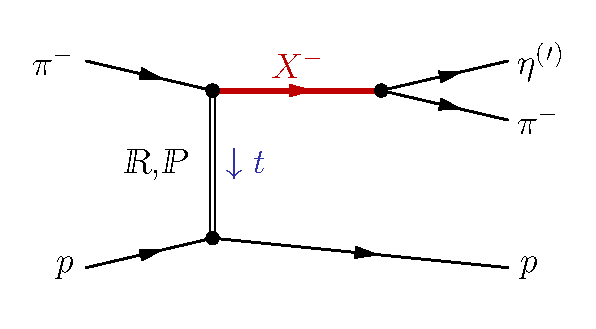
\includegraphics[width=0.5\textwidth]{diffractive_dissociation_x_etaprimepi_charged_p}%
  \caption{Diffractive scattering of a beam pion off a target proton
  mediated by Reggeon exchange.  In this scattering process, an
  intermediate state~$X^-$ with well-defined quantum numbers is
  produced, which in the example given here decays into the
  \etaOrPrPim channel.}%
  \label{fig:diffractive_etaprimepi}%
\end{figure}

The analysis is based on the measured intensity distribution, \ie the
number density of events, which is decomposed into partial-wave
amplitudes:\footnote{This is the simplest possible formula, were we
assume that the effect of the target spin is negligible and that all
partial wave amplitudes are fully coherent.}
\begin{equation}
  \label{eq:diffraction_intensity}
  \mathcal{I}(\Omega; w, t)
  = \frac{\dif{N}}{\dif{w}\, \dif{t}\, \dif{\Omega}}
  = \Abs[3]{\sum_{\ell m}^\infty \mathcal{T}_{\ell\, m}(w, t)\, Y_\ell^m(\Omega)}^2
  = \sum_{\substack{\ell m \\ \ell' m'}}^\infty Y_\ell^m(\Omega)\, \varrho^{\ell\, \ell'}_{m\, m'}(w, t)\, Y_{\ell'}^{m' *}(\Omega).
\end{equation}
Here, $N$~is the (acceptance-corrected) number of measured events,
$w$~is the invariant mass of the two-(pseudo)scalar system, $t$~is the
squared four-momentum transferred from the beam to the target
particle, and $\Omega = (\theta, \phi)$ is the direction of one of the
two (pseudo)scalar mesons the~$X$ decays into, measured in the
Gottfried-Jackson rest frame of~$X$.  The $\mathcal{T}_{\ell\, m}(w,
t)$ are the partial-wave amplitudes that correspond to an intermediate
state with a spin given by the relative orbital angular
momentum~$\ell$ between the two-(pseudo)scalar mesons and a spin
projection~$m$ \wrt the beam axis.  The partial-wave amplitudes form
the spin-density matrix of~$X$:
\begin{equation}
  \label{eq:diffraction_spin_dens_def}
  \varrho^{\ell\, \ell'}_{m\, m'}(w, t)
  = \mathcal{T}_{\ell\, m}(w, t)\, \mathcal{T}_{\ell'\, m'}^*(w, t),
\end{equation}
which by definition is Hermitian.  The angular distribution of the
$X$~decay products is given by the spherical harmonics
$Y_\ell^m(\Omega)$~\cite{wikipedia:sphericalHarm}, which are defined
by\footnote{See Eq.~(1) in Sec.~5.2 of
\refCite{Varshalovich:1988krb}.}
\begin{equation}
  \label{eq:spherical_harm_def}
  Y_\ell^m(\Omega)
  = \dUnderbrace{\sqrt{\frac{(2 \ell + 1)}{4 \pi}\, \frac{(\ell -m)!}{(\ell + m)!}}\, P_\ell^m(\cos\theta)}{= Y_\ell^m(\theta, 0)}\, e^{\imag\, m\, \phi},
\end{equation}
For convenience, we introduce the real-valued functions
\begin{equation}
  \label{eq:small_y_def}
  y_\ell^m(\theta)
  \equiv Y_\ell^m(\theta, 0)
  \quad\text{so that}\quad
  Y_\ell^m(\theta, \phi)
  = y_\ell^m(\theta)\, e^{\imag\, m\, \phi}.
\end{equation}
The spherical harmonics are special cases of the
$D$-functions~\cite{wikipedia:wignerD}, \ie\footnote{See Eq.~(37) in
Sec.~5.2.7 of \refCite{Varshalovich:1988krb}.}
\begin{equation}
  \label{eq:spherical_harm_wigner_d}
  Y_\ell^m(\Omega)
  = \sqrt{\frac{2 \ell + 1}{4 \pi}}\, D^{\ell *}_{m 0}(\phi, \theta, 0)
  \quad\text{and in particular}\quad
  y_\ell^m(\theta)
  = \sqrt{\frac{2 \ell + 1}{4 \pi}}\, d^\ell_{m 0}(\theta).
\end{equation}

In a partial-wave analysis, the partial-wave amplitudes
$\mathcal{T}_{\ell\, m}$, which contain the information about the
produced resonances~$X$, are determined by fitting the intensity model
in \cref{eq:diffraction_intensity} to the measured
$\Omega$~distribution in narrow $(w, t)$ cells.  Within each kinematic
cell, $\mathcal{T}_{\ell\, m}$ is treated as constant.  To simplify
notation, we hence will omit the~$w$ and $t$~dependencies in all
formulas below.

In addition to the partial-wave analysis, which decomposes the
\emph{amplitudes} into spherical harmonics, we can exploit the fact
that the $Y_\ell^m(\Omega)$ constitute a complete orthonormal set of
base functions on the surface of a unit sphere, \ie they fullfil the
completeness relation\footnote{See Eq.~(1) in Sec.~5.6.1 of
\refCite{Varshalovich:1988krb}.}
\begin{equation}
  \label{eq:spherical_harm_complete}
  \sum_{\ell m}^\infty Y_\ell^m(\Omega)\, Y_\ell^{m *}(\Omega')
  = \delta(\phi' - \phi)\, \delta(\theta' - \theta)
\end{equation}
and the orthonormality relation\footnote{%
Throughout the text, we use
\begin{equation}
  \int_{-1}^{+1}\!\!\! \dif{\cos\theta} \int_{-\pi}^{+\pi}\!\!\! \dif{\phi}
  = \int_{4 \pi}\!\!\! \dif{\Omega}.
\end{equation}
}\footnote{See Eq.~(2) in Sec.~5.6.1 of
\refCite{Varshalovich:1988krb}.}
\begin{equation}
  \label{eq:spherical_harm_orthonorm}
  \int_{4 \pi}\!\!\! \dif{\Omega}\, Y_\ell^m(\Omega)\, Y_{\ell'}^{m' *}(\Omega)
  = \delta_{\ell \ell'}\, \delta_{m m'},
\end{equation}
and instead decompose the \emph{intensity} into spherical harmonics.

Using \cref{eq:gen_fourier_series,eq:expansion_coefficient} we
obtain:\footnote{The expansion into a series of spherical harmonics is
also referred to as Laplace series~\cite{MathWorld:LaplaceSeries}.}
\begin{equation}
  \label{eq:diffraction_intensity_moments}
  \mathcal{I}(\Omega)
  = \sum_{L M}^\infty H(L, M)\, Y_L^M(\Omega),
\end{equation}
with the moments\footnote{Note that in
\cref{sec:diffraction:moments_norm}, we will introduce a different
normalization for $H(L, M)$ (see \cref{eq:diffraction_moments_norm}).}
\begin{equation}
  \label{eq:diffraction_moments}
  H(L, M)
  = \int_{4 \pi}\!\!\! \dif{\Omega}\, \mathcal{I}(\Omega)\, Y_L^{M *}(\Omega).
\end{equation}
It is important to note that although
\cref{eq:diffraction_intensity_moments} and
\cref{eq:diffraction_intensity} use the same basis functions, the two
represent different decompositions.  In
\cref{eq:diffraction_intensity} the amplitudes are decomposed into
spherical harmonics, \ie partial-wave amplitudes, whereas in
\cref{eq:diffraction_intensity_moments} the intensity is decomposed.
Whereas the former decomposition is based on a physics model of the
reaction, the moment decomposition is purely mathematical.  An
advantage of the moment decomposition is that it is unique, whereas
the partial-wave decomposition may have mathematical as well as
statistical ambiguities (see \eg\ \refCite{Chung:1997qd}).  Another
advantage of the moment decomposition is that the moments can be
rather easily calculated from the data, which will be discussed in
\cref{sec:diffraction:moments_data}.  The downside of this approach is
that the physics interpretation of the moments is difficult because
they are only indirectly related to the partial-wave amplitudes.  This
will be discussed in more detail in \cref{sec:diffraction:moments_pw}.


\subsection{Relation between moments and partial-wave amplitudes}%
\label{sec:diffraction:moments_pw}

In order to relate the partial-wave amplitudes~$\mathcal{T}_{\ell\,
m}$ and the moments~$H(L, M)$ we express the moments in terms of
spin-density elements using the relation\footnote{See Eq.~(A.15) in
\refCite{Chung:1971ri}.}
\begin{equation}
  \label{eq:spherical_harm_prod}
  Y_{\ell'}^{m' *}(\Omega)\, Y_{\ell}^m(\Omega)
  = \sum_{L M}^\infty \sqrt{\frac{2 L + 1}{4 \pi}}\, \sqrt{\frac{2 \ell' + 1}{2 \ell + 1}}\, \clebsch{\ell'}{0}{L}{0}{\ell}{0}\, \clebsch{\ell'}{m'}{L}{M}{\ell}{m}\, Y_L^M(\Omega).
\end{equation}
Here, \clebsch{j_1}{m_1}{j_2}{m_2}{J}{M} are the Clebsch-Gordan
coefficients for the coupling of the spin states $\ket{j_1\; m_1}$
and~$\ket{j_2\; m_2}$ to $\ket{J\; M}$.  Note that the Clebsch-Gordan
coefficient \clebsch{\ell'}{0}{L}{0}{\ell}{0} requires
that\footnote{See Eq.~(32) in Sec.~8.5.2 of
\refCite{Varshalovich:1988krb}.}
\begin{equation}
  \label{eq:ang_mom_sum}
  \ell' + L + \ell
  = \text{even}.
\end{equation}
Inserting \cref{eq:spherical_harm_prod} into
\cref{eq:diffraction_intensity}, yields
\begin{equation}
  \mathcal{I}(\Omega)
  = \sum_{L M}^\infty \sqrt{\frac{2 L + 1}{4 \pi}} \sum_{\substack{\ell m \\ \ell' m'}}^\infty
  \sqrt{\frac{2 \ell' + 1}{2 \ell + 1}}\, \clebsch{\ell'}{0}{L}{0}{\ell}{0}\, \clebsch{\ell'}{m'}{L}{M}{\ell}{m}\,
  \varrho^{\ell\, \ell'}_{m\, m'}\, Y_L^M(\Omega).
\end{equation}
Comparing with \cref{eq:diffraction_intensity_moments}, we see
that\footnote{Note that in \cref{sec:diffraction:moments_norm}, we
will introduce a different normalization for $H(L, M)$ (see
\cref{eq:diffraction_moments_pw_norm}).}
\begin{equation}
  \label{eq:diffraction_moments_pw}
  H(L, M)
  = \sqrt{\frac{2 L + 1}{4 \pi}} \sum_{\substack{\ell m \\ \ell' m'}}^\infty
  \sqrt{\frac{2 \ell' + 1}{2 \ell + 1}}\,
  \clebsch{\ell'}{0}{L}{0}{\ell}{0}\, \clebsch{\ell'}{m'}{L}{M}{\ell}{m}\,
  \varrho^{\ell\, \ell'}_{m\, m'}.
\end{equation}

It is important to note that we can always calculate all moments from
a given set of partial-wave amplitudes using
\cref{eq:diffraction_moments_pw}.  However, in general the converse is
not true because there are unphysical sets of moments that do not
correspond to a partial-wave decomposition and even for a physical set
of moments we need to solve a system of quadratic equations in the
partial-wave amplitudes given by
\cref{eq:diffraction_moments_pw,eq:diffraction_spin_dens_def}, which
may contain ambiguities.

From \cref{eq:diffraction_moments_pw} it is clear that the moments are
linear combinations of spin-density matrix elements, \ie of
intensities and interference terms of the partial-wave amplitudes
$\mathcal{T}_{\ell\, m}$.  The equation also shows that~$L$ and~$M$
are only indirectly linked to the physical angular momentum quantum
numbers of the two-body system.  For given~$L$, the Clebsch-Gordan
coefficients limit the sum to those partial waves, for which $\ell' +
L + \ell = \text{even}$ (see \cref{eq:ang_mom_sum}), $\abs{\ell' - L}
\leq \ell \leq \ell' + L$, and $m = m' + M$.  This means that if the
partial-wave amplitudes vanish for $\ell, \ell' > \ell_\text{max}$ the
moments~$H(L, M)$ will vanish $L > 2 \ell_\text{max}$.

Alternatively, we can derive \cref{eq:diffraction_moments_pw} by
inserting \cref{eq:diffraction_intensity} into
\cref{eq:diffraction_moments} and using\footnote{This is the complex
conjugate of Eq.~(4) in Sec.~5.9.1 of \refCite{Varshalovich:1988krb}.}
\begin{equation}
  \label{eq:spherical_harm_clebsch}
  \int_{4 \pi}\!\!\! \dif{\Omega}\,
  Y_{\ell'}^{m' *}(\Omega)\, Y_L^{M *}(\Omega)\, Y_{\ell}^m(\Omega)
  = \sqrt{\frac{2 \ell' + 1}{4 \pi}}\, \sqrt{\frac{2 L + 1}{2 \ell + 1}}\, \clebsch{\ell'}{0}{L}{0}{\ell}{0}\, \clebsch{\ell'}{m'}{L}{M}{\ell}{m}.
\end{equation}
Doing so, we obtain
\begin{equation}
  H(L, M)
  = \sum_{\substack{\ell m \\ \ell' m'}}^\infty
  \varrho^{\ell\, \ell'}_{m\, m'}\,
  \int_{4 \pi}\!\!\! \dif{\Omega}\,
  Y_\ell^m(\Omega)\,
  Y_{\ell'}^{m' *}(\Omega)\,
  Y_L^{M *}(\Omega),
\end{equation}
which is equivalent to \cref{eq:diffraction_moments_pw}.


\subsection{Normalization of moments}%
\label{sec:diffraction:moments_norm}

In order to derive a more practical normalization of the moments, it
is instructive to look at the lowest moment $H(0, 0)$, which is a
special case.  With
\cref{eq:diffraction_moments,eq:diffraction_moments_pw},
$Y_0^0(\Omega) = 1 / \sqrt{4 \pi}$, and
\begin{equation}
  \clebsch{\ell'}{m'}{0}{0}{\ell}{m}
  = \delta_{\ell \ell'}\, \delta_{m m'}
\end{equation}
we get
\begin{equation}
  H(0, 0)
  = \frac{1}{\sqrt{4 \pi}}\, \int_{4 \pi}\!\!\! \dif{\Omega}\, \mathcal{I}(\Omega)
  = \sqrt{\frac{2 L + 1}{4 \pi}} \sum_{\substack{\ell m \\ \ell' m'}}^\infty \varrho^{\ell\, \ell}_{m\, m}.
\end{equation}
This means, up to a factor of $1 / \sqrt{4 \pi}$, $H(0, 0)$ is the
integral of the intensity over the phase space, which is identical to
the sum of all partial-wave intensities.

In order to make $H(0, 0)$ identical to the intensity integral and the
sum of all partial-wave intensities, it is customary to change the
normalization of the moments using the replacement
\begin{equation}
  H(L, M)
  \to \sqrt{\frac{4 \pi}{2 L + 1}}\, H(L, M).
\end{equation}
Applying the above,
\cref{eq:diffraction_intensity_moments,eq:diffraction_moments} become
\begin{equation}
  \label{eq:diffraction_intensity_moments_norm}
  \mathcal{I}(\Omega)
  = \sum_{L M}^\infty \sqrt{\frac{2 L + 1}{4 \pi}}\, H(L, M)\, Y_L^M(\Omega),
\end{equation}
and
\begin{equation}
  \label{eq:diffraction_moments_norm}
  H(L, M)
  = \sqrt{\frac{4 \pi}{2 L + 1}}\, \int_{4 \pi}\!\!\! \dif{\Omega}\, \mathcal{I}(\Omega)\, Y_L^{M *}(\Omega).
\end{equation}
Using the relation between the spherical harmonics and the Wigner
$D$-functions in \cref{eq:spherical_harm_wigner_d},
\cref{eq:diffraction_intensity_moments_norm,eq:diffraction_moments_norm}
become identical to Eqs.~(6) and~(9) in \refCite{Chung:1997qd}.

Similarly, \cref{eq:diffraction_moments_pw} becomes
\begin{equation}
  \label{eq:diffraction_moments_pw_norm}
  H(L, M)
  = \sum_{\substack{\ell m \\ \ell' m'}}^\infty
  \sqrt{\frac{2 \ell' + 1}{2 \ell + 1}}\,
  \clebsch{\ell'}{0}{L}{0}{\ell}{0}\, \clebsch{\ell'}{m'}{L}{M}{\ell}{m}\,
  \varrho^{\ell\, \ell'}_{m\, m'}.
\end{equation}

For the remainder of this section we will use the moments defined in
\cref{eq:diffraction_intensity_moments_norm,eq:diffraction_moments_norm,eq:diffraction_moments_pw_norm}, for which in particular
\begin{equation}
  \label{eq:diffraction_moment_00_pw}
  H(0, 0)
  = \int_{4 \pi}\!\!\! \dif{\Omega}\, \mathcal{I}(\Omega)
  = \sum_{\substack{\ell m \\ \ell' m'}}^\infty \varrho^{\ell\, \ell}_{m\, m}.
\end{equation}


\subsection{Symmetry properties of moments}%
\label{sec:diffraction:moments_sym}

Since the moments are defined by the spherical harmonics (see
\cref{eq:diffraction_moments_norm}), they inherit the symmetry properties
of the spherical harmonics.  From\footnote{See Eq.~(1) in Sec.~5.4 of
\refCite{Varshalovich:1988krb}.}
\begin{equation}
  \label{eq:spherical_harm_sym}
  Y_L^{M *}(\Omega)
  = (-1)^M\, Y_L^{(-M)}(\Omega)
\end{equation}
it follows that
\begin{equation}
  \label{eq:diffraction_moment_sym_1}
  H^*(L, M)
  = \sqrt{\frac{4 \pi}{2 L + 1}}\, \int_{4 \pi}\!\!\! \dif{\Omega}\, \mathcal{I}(\Omega)\, Y_L^M(\Omega)
  = (-1)^M \sqrt{\frac{4 \pi}{2 L + 1}}\, \int_{4 \pi}\!\!\! \dif{\Omega}\, \mathcal{I}(\Omega)\, Y_L^{(-M) *}(\Omega)
  = (-1)^M\, H(L, -M).
\end{equation}

Alternatively, we can derive \cref{eq:diffraction_moment_sym_1} by
using \cref{eq:diffraction_moments_pw_norm} plus the fact that the
spin-density matrix is Hermitian,
\ie
\begin{equation}
  \rBrk[1]{\varrho^{\ell\, \ell'}_{m\, m'}}^*
  = \varrho^{\ell'\, \ell}_{m'\, m},
\end{equation}
and that the Clebsch-Gordan coefficients have the symmetry
property\footnote{See Eq.~(10) in Sec.~8.4.3 of
\refCite{Varshalovich:1988krb}.}
\begin{equation}
  \label{eq:clebsch_sym}
  \clebsch{\ell'}{m'}{L}{M}{\ell}{m}
  = \rdUnderbrace{(-1)^{\ell' + L - \ell}}{\equalUsing{$\mathclap{\text{\cref{eq:ang_mom_sum}}}$}\quad 1}\,
  \clebsch{L}{M}{\ell'}{m'}{\ell}{m}
  = (-1)^{L - M}\, \sqrt{\frac{2 \ell + 1}{2 \ell' + 1}}\, \clebsch{\ell}{m}{L}{-M}{\ell'}{m'}.
\end{equation}
Doing so, we get
\begin{align}
  H^*(L, M)
  ={}& \sum_{\substack{\ell m \\ \ell' m'}}^\infty
    \sqrt{\frac{2 \ell' + 1}{2 \ell + 1}}\,
    (-1)^{L - 0}\, \sqrt{\frac{2 \ell + 1}{2 \ell' + 1}}\, \clebsch{\ell}{0}{L}{0}{\ell'}{0}\,
    (-1)^{L - M}\, \sqrt{\frac{2 \ell + 1}{2 \ell' + 1}}\, \clebsch{\ell}{m}{L}{-M}{\ell'}{m'}\,
    \varrho^{\ell'\, \ell}_{m'\, m} \notag
  \\
  ={}& \dUnderbrace{(-1)^{2 L - M}}{= (-1)^M}
  \sum_{\substack{\ell m \\ \ell' m'}}^\infty
  \sqrt{\frac{2 \ell + 1}{2 \ell' + 1}}\,
  \clebsch{\ell}{0}{L}{0}{\ell'}{0}\, \clebsch{\ell}{m}{L}{-M}{\ell'}{m'}\,
  \varrho^{\ell'\, \ell}_{m'\, m}
  \\
  \equalUsing{$\mathclap{\substack{\displaystyle{\ell \leftrightarrow \ell'} \\ \displaystyle{m \leftrightarrow m'}}}$}{}& \quad
  (-1)^M\, H(L, -M),
\end{align}
where in the last step we rearranged the terms in the sum and compared
to \cref{eq:diffraction_moments_pw_norm}.

The symmetry relation in \cref{eq:diffraction_moment_sym_1} ensures
that the intensity function in
\cref{eq:diffraction_intensity_moments_norm} is real-valued:
\begin{flalign}
  \mathcal{I}(\Omega)
  ={}& \sum_{L = 0}^\infty \sum_{M = -L}^{+L} \sqrt{\frac{2 L + 1}{4 \pi}}\, H(L, M)\, Y_L^M(\Omega) && \notag
  \\
  ={}& \sum_{L = 0}^\infty \sqrt{\frac{2 L + 1}{4 \pi}} \sBrk[4]{\rdUnderbrace{\sum_{M = -L}^{-1} H(L, M)\, Y_L^M(\Omega)}%
    {= \sum_{M = +1}^{+L} H(L, -M)\, Y_L^{(-M)}(\Omega)
    \equalUsingTwo{\cref{eq:spherical_harm_sym}}{\cref{eq:diffraction_moment_sym_1}} (-1)^M\, H^*(L, M)\, (-1)^M\, Y_L^{M *}(\Omega)}
    + H(L, 0)\, Y_L^0(\Omega) + \sum_{M = +1}^{+L} H(L, M)\, Y_L^M(\Omega)} && \notag
  \\
  ={}& \sum_{L = 0}^\infty \sqrt{\frac{2 L + 1}{4 \pi}} \sBrk[4]{H(L, 0)\, Y_L^0(\Omega) + \sum_{M = +1}^{+L}
  \rdUnderbrace{\cBrk{H(L, M)\,Y_L^M(\Omega) + H^*(L, M)\,Y_L^{M *}(\Omega)}}{= 2 \Re{H(L, M)\, Y_L^M(\Omega)}}} && \notag
  \\
  \label{eq:diffraction_intensity_moments_general}
  ={}& \sum_{L = 0}^\infty \sqrt{\frac{2 L + 1}{4 \pi}} \sum_{M = 0}^{L} (2 - \delta_{M 0})\, \Re{H(L, M)\, Y_L^M(\Omega)}. &&
\end{flalign}
For the last step, we have used that $Y_L^0(\Omega)$ and hence also
$H(L, 0)$ are real-valued by construction.  Due to the above, we only
have to calculate the moments with $M \geq 0$.

In addition to the symmetry properties of the spherical harmonics, we
can also exploit the symmetry properties of the $X$~spin-density
matrix.  Since the scattering process is invariant under parity, we
have\footnote{See Eq.~2.7 in \refCite{Chung:1974fq}.}
\begin{equation}
  \label{eq:diffraction_spin_dens_parity_general}
  \varrho^{\ell\, \ell'}_{m\, m'}
  = P\, P'\, (-1)^{\ell - \ell'}\, (-1)^{m - m'}\, \varrho^{\ell'\, \ell}_{{-m}\, {-m'}}.
\end{equation}
Here $\ell^P$ and $(\ell')^{P'}$ are two spin-parity states of~$X$.
For the two-body decay $X \to 1 + 2$, the intrinsic parity of~$X$ is
given by
\begin{equation}
  P
  = P_1\, P_2\, (-1)^\ell.
\end{equation}
Assuming that $X$~decays into two daughter particles with identical
parity, \eg two pseudoscalars such as $\etaOrPr \pi$,
\cref{eq:diffraction_spin_dens_parity_general} simplifies to
\begin{equation}
  \label{eq:diffraction_spin_dens_parity}
  \varrho^{\ell\, \ell'}_{m\, m'}
  = (-1)^{m - m'}\, \varrho^{\ell'\, \ell}_{{-m}\, {-m'}}.
\end{equation}

Using this together with
\cref{eq:diffraction_moments_pw_norm} and the symmetry
property\footnote{See Eq.~(11) in Sec.~8.4.3 of
\refCite{Varshalovich:1988krb}.}
\begin{equation}
  \label{eq:clebsch_sym2}
  \clebsch{\ell'}{m'}{L}{M}{\ell}{m}
  = \rdUnderbrace{(-1)^{\ell' + L - \ell}}{\equalUsing{$\mathclap{\text{\cref{eq:ang_mom_sum}}}$}\quad 1}\,
  \clebsch{\ell'}{-m'}{L}{-M}{\ell}{-m}
\end{equation}
of the Clebsch-Gordan coefficients, we get
\begin{align}
  H(L, -M)
  ={}& \sum_{\substack{\ell m \\ \ell' m'}}^\infty
  \sqrt{\frac{2 \ell' + 1}{2 \ell + 1}}\,
  \clebsch{\ell'}{0}{L}{0}{\ell}{0}\, \clebsch{\ell'}{-m'}{L}{M}{\ell}{-m}\,
  (-1)^{m - m'}\, \varrho^{\ell\, \ell'}_{{-m}\, {-m}'} \notag
  \\
  \label{eq:diffraction_moment_sym_2}
  \equalUsing{$\mathclap{\substack{\displaystyle{m \to -m} \\ \displaystyle{m' \to -m'}}}$}{}& \quad
  (-1)^M\, H(L, M),
\end{align}
where in the last step, we used that the second Clebsch-Gordan
coefficient enforces $m' - M = m$,\footnote{Therefore, $(-1)^{m - m'}
= (-1)^{m' - m} = (-1)^M$.} rearranged the terms in the sum, and
compared to \cref{eq:diffraction_moments_pw_norm}.

From \cref{eq:diffraction_moment_sym_1,eq:diffraction_moment_sym_2} follows that
\begin{equation}
  H(L, M)
  = H^*(L, M),
\end{equation}
\ie all moments must be real-valued.  Inserting
\cref{eq:small_y_def,eq:diffraction_moments_norm} on both sides, we
obtain
\begin{align}
  \sqrt{\frac{4 \pi}{2 L + 1}}\, \int_{4 \pi}\!\!\! \dif{\Omega}\, \mathcal{I}(\Omega)\, Y_L^{M *}(\Omega)
  \mustBeEq{}&
  \sqrt{\frac{4 \pi}{2 L + 1}}\, \int_{4 \pi}\!\!\! \dif{\Omega}\, \mathcal{I}(\Omega)\, Y_L^M(\Omega) \\
  \sqrt{\frac{4 \pi}{2 L + 1}}\, \int_{4 \pi}\!\!\! \dif{\Omega}\, \mathcal{I}(\Omega)\, y_L^M(\theta) \sBrk{\cos(M \phi) - \imag \sin(M \phi)}
  \mustBeEq{}&
  \sqrt{\frac{4 \pi}{2 L + 1}}\, \int_{4 \pi}\!\!\! \dif{\Omega}\, \mathcal{I}(\Omega)\, y_L^M(\theta) \sBrk{\cos(M \phi) + \imag \sin(M \phi)}.
\end{align}
Consequently,
\begin{align}
  \label{eq:diffraction_moments_real}
  H(L, M)
  ={}& \sqrt{\frac{4 \pi}{2 L + 1}}\, \int_{4 \pi}\!\!\! \dif{\Omega}\, \mathcal{I}(\Omega)\, y_L^M(\theta)\, \cos(M\, \phi)
  \intertext{and}
  \label{eq:diffraction_moments_imag}
  0
  ={}& \sqrt{\frac{4 \pi}{2 L + 1}}\, \int_{4 \pi}\!\!\! \dif{\Omega}\, \mathcal{I}(\Omega)\, y_L^M(\theta)\, \sin(M\, \phi).
\end{align}

We can also rewrite \cref{eq:diffraction_intensity_moments_general}:
\begin{align}
  \mathcal{I}(\Omega)
  ={}& \sum_{L = 0}^\infty \sqrt{\frac{2 L + 1}{4 \pi}} \sum_{M = 0}^{L} (2 - \delta_{M 0})\, H(L, M)\, \Re{Y_L^M(\Omega)} \notag
  \\
  \label{eq:diffraction_intensity_moments_real}
  ={}& \sum_{L = 0}^\infty \sqrt{\frac{2 L + 1}{4 \pi}} \sum_{M = 0}^{L} (2 - \delta_{M 0})\, H(L, M)\, y_L^M(\theta)\, \cos(M\, \phi).
\end{align}
This is identical to Eq.~(13) in \refCite{Chung:1997qd}.


\subsection{Reflectivity basis}%
\label{sec:diffraction:reflectivity}

It is often advantageous to express the intensity distribution in
\cref{eq:diffraction_intensity} in the reflectivity basis, \ie using
the reflectivity states of~$X$
\begin{equation}
  \label{eq:diffraction_refl_def}
  \ket{\refl, \ell, m}
  \equiv \mathcal{N}_m \sBrk[2]{\ket{\ell, m} - \refl\, (-1)^m\, \ket{\ell, {-m}}},
\end{equation}
which are eigenstates of the reflection operator~$\Pi_y$ through the
production plane that is spanned by the momenta of the beam particle
and~$X$.  The relative sign of the terms in
\cref{eq:diffraction_refl_def} has been chosen such that for a
pseudoscalar beam particle the eigenvalues~$\refl = \pm$ of~$\Pi_y$,
\ie the \emph{reflectivities}, correspond to the \emph{naturality} of
the exchange particle in the scattering process.  The normalization
factor
\begin{equation}
  \label{eq:refl_norm}
  \mathcal{N}_m
  = \begin{cases*}
      1 / \sqrt{2} & for $m > 0$, \\
      1 / 2        & for $m = 0$, \\
      0            & for $m < 0$
    \end{cases*}
\end{equation}
ensures that the multiplicity of $2 \ell + 1$ of the spin states is
conserved by constraining~$m$ to be non-negative.  It is important to
note that the definition in \cref{eq:diffraction_refl_def} forbids
positive-reflectivity states with $m = 0$.

The reflectivity basis is implemented by introducing the functions
\begin{equation}
  \label{eq:diffraction_spherical_harm_refl}
  \prescript{(\refl)}{}{Y}_\ell^m(\Omega)
  \equiv \mathcal{N}_m \sBrk[2]{Y_\ell^m(\Omega) - \refl\, (-1)^m\, Y_\ell^{(-m)}(\Omega)}.
\end{equation}
Note that with \cref{eq:spherical_harm_sym} and the definition of the
spherical harmonics in \cref{eq:spherical_harm_def,eq:small_y_def}, it
follows from \cref{eq:diffraction_spherical_harm_refl} that
\begin{equation}
  \prescript{(+)}{}{Y}_\ell^m(\Omega)
  = 2 \imag\, \mathcal{N}_m\, y_\ell^m(\theta)\, \sin(m\, \phi)
  \quad\text{and}\quad
  \prescript{(-)}{}{Y}_\ell^m(\Omega)
  = 2 \mathcal{N}_m\, y_\ell^m(\theta)\, \cos(m\, \phi),
\end{equation}
\ie $\prescript{(+)}{}{Y}_\ell^m(\Omega)$ is purely imaginary and
$\prescript{(-)}{}{Y}_\ell^m(\Omega)$ purely real.

Replacing $Y_\ell^m(\Omega)$ in \cref{eq:diffraction_intensity} by
\cref{eq:diffraction_spherical_harm_refl} and using the fact that
amplitudes with opposite reflectivities do not interfere, we obtain
\begin{equation}
  \label{eq:diffraction_intensity_refl}
  \mathcal{I}(\Omega)
  = \sum_{\refl = \pm} \Abs[3]{\sum_{\ell m}^\infty \prescript{(\refl)}{}{\mathcal{T}}_{\!\ell\, m}\, \prescript{(\refl)}{}{Y}_\ell^m(\Omega)}^2
  = \sum_{\refl = \pm} \sum_{\substack{\ell m \\ \ell' m'}}^\infty
  \prescript{(\refl)}{}{Y}_\ell^m(\Omega)\, \prescript{(\refl)}{}{\varrho}^{\ell\, \ell'}_{m\, m'}\, \prescript{(\refl)}{}{Y}_{\ell'}^{m' *}(\Omega),
\end{equation}
where we have introduced the spin-density matrix of~$X$,
\begin{equation}
  \label{eq:diffraction_refl_spin-dens}
  \prescript{(\refl)}{}{\varrho}^{\ell\, \ell'}_{m\, m'}
  = \prescript{(\refl)}{}{\mathcal{T}}_{\!\ell\, m}\, \prescript{(\refl)}{}{\mathcal{T}}_{\!\ell'\, m'}^*,
\end{equation}
in the reflectivity basis analogous to
\cref{eq:diffraction_spin_dens_def}.

In order to relate the partial-wave
amplitudes~$\prescript{(\refl)}{}{\mathcal{T}}_{\!\ell\, m}$ and the
moments~$H(L, M)$ we insert \cref{eq:diffraction_spherical_harm_refl}
into \cref{eq:diffraction_intensity_refl} and use
\cref{eq:spherical_harm_prod}:
\begin{align}
  \mathcal{I}(\Omega)
  ={}&
    \sum_{\refl = \pm} \sum_{\substack{\ell m \\ \ell' m'}}^\infty
    \prescript{(\refl)}{}{\varrho}^{\ell\, \ell'}_{m\, m'}\,
    \mathcal{N}_m\, \mathcal{N}_{m'}
    \sBrk[2]{Y_\ell^m(\Omega) - \refl\, (-1)^m\, Y_\ell^{(-m)}(\Omega)}
    \sBrk[2]{Y_{\ell'}^{m' *}(\Omega) - \refl\, (-1)^{m'}\, Y_{\ell'}^{(-m') *}(\Omega)}
  \\
  ={}& \begin{multlined}[t][0.85\columnwidth]
    \sum_{\refl = \pm} \sum_{\substack{\ell m \\ \ell' m'}}^\infty
    \prescript{(\refl)}{}{\varrho}^{\ell\, \ell'}_{m\, m'}\,
    \sum_{L M}^\infty \sqrt{\frac{2 L + 1}{4 \pi}}\, \sqrt{\frac{2 \ell' + 1}{2 \ell + 1}}\, \clebsch{\ell'}{0}{L}{0}{\ell}{0} \\
    \shoveleft{\times \mathcal{N}_m\, \mathcal{N}_{m'}\, \Big[ \clebsch{\ell'}{m'}{L}{M}{\ell}{m}                       - \refl\, (-1)^{m'}\, \clebsch{\ell'}{-m'}{L}{M}{\ell}{m}} \\
      - \refl\, (-1)^m\, \clebsch{\ell'}{m'}{L}{M}{\ell}{-m} + (-1)^{m + m'}\, \clebsch{\ell'}{-m'}{L}{M}{\ell}{-m} \Big]\,
    Y_L^M(\Omega).
  \end{multlined}
\end{align}
We rewrite the last Clebsch-Gordan coefficient in the square bracket
using the symmetry relation in \cref{eq:clebsch_sym2} and the fact
that $(-1)^{m + m'} = (-1)^{2m}\, (-1)^{m' - m} = (-1)^M$ because this
Clebsch-Gordan coefficient enforces that $m' - M = m$.  With this we
arrive at
\begin{multline}
  \mathcal{I}(\Omega)
  = \sum_{L M}^\infty \sqrt{\frac{2 L + 1}{4 \pi}}
  \sum_{\refl = \pm} \sum_{\substack{\ell m \\ \ell' m'}}^\infty
  \mathcal{N}_m\, \mathcal{N}_{m'}\,
  \sqrt{\frac{2 \ell' + 1}{2 \ell + 1}}\,
  \clebsch{\ell'}{0}{L}{0}{\ell}{0}
  \\
  \times \Big[
    \clebsch{\ell'}{m'}{L}{M}{\ell}{m}
    + (-1)^M\, \clebsch{\ell'}{m'}{L}{-M}{\ell}{m} \\
    - \refl\, (-1)^{m'}\, \clebsch{\ell'}{-m'}{L}{M}{\ell}{m}
    - \refl\, (-1)^m\, \clebsch{\ell'}{m'}{L}{M}{\ell}{-m} \Big]
  \prescript{(\refl)}{}{\varrho}^{\ell\, \ell'}_{m\, m'}\,
  Y_L^M(\Omega).
\end{multline}
Comparing with \cref{eq:diffraction_intensity_moments_norm} we see
that
\begin{multline}
  \label{eq:diffraction_moments_pw_refl_norm}
  H(L, M)
  = \sum_{\refl = \pm} \sum_{\substack{\ell m \\ \ell' m'}}^\infty
  \mathcal{N}_m\, \mathcal{N}_{m'}\,
  \sqrt{\frac{2 \ell' + 1}{2 \ell + 1}}\,
  \clebsch{\ell'}{0}{L}{0}{\ell}{0} \\
  \times \Big[
    \clebsch{\ell'}{m'}{L}{M}{\ell}{m}
    + (-1)^M\, \clebsch{\ell'}{m'}{L}{-M}{\ell}{m} \\
    - \refl\, (-1)^{m'}\, \clebsch{\ell'}{-m'}{L}{M}{\ell}{m}
    - \refl\, (-1)^m\, \clebsch{\ell'}{m'}{L}{M}{\ell}{-m} \Big]
  \prescript{(\refl)}{}{\varrho}^{\ell\, \ell'}_{m\, m'},
\end{multline}
which is identical to Eqs.~(29) and~(31) in \refCite{Chung:1997qd}.
It is important to note that each moment is an incoherent sum of
contributions from both reflectivities, \ie the moments do not
separate these contributions.
\Cref{eq:diffraction_moments_pw_refl_norm} is the equivalent of
\cref{eq:diffraction_moments_pw_norm} in the reflectivity basis.

Using the above, we can calculate the lowest moment in the
reflectivity basis:
\begin{align}
  H(0, 0)
  ={}& \begin{multlined}[t]
    \sum_{\refl = \pm} \sum_{\substack{\ell m \\ \ell' m'}}^\infty
    \sqrt{\frac{2 \ell' + 1}{2 \ell + 1}}\,
    \delta_{\ell \ell'}
    \\
    \times \rdUnderbrace{\mathcal{N}_m\, \mathcal{N}_{m'} \sBrk[2]{%
      \delta_{\ell \ell'}\, \delta_{m m'}
      + \delta_{\ell \ell'}\, \delta_{m m'}
      - \refl\, (-1)^{m'}\, \delta_{\ell \ell'}\, \delta_{m (-m')}
      - \refl\, (-1)^m\, \delta_{\ell \ell'}\, \delta_{(-m) m'}}}%
      {= \delta_{\ell \ell'}\, \delta_{m m'} \times
      \begin{cases*}
        \frac{1}{2}\, (1 + 1)                 & for $m > 0$, \\
        \frac{1}{4}\, (1 + 1 - \refl - \refl) & for $m = 0$
      \end{cases*}}
    \prescript{(\refl)}{}{\varrho}^{\ell\, \ell'}_{m\, m'}
  \end{multlined} \notag
  \\
  \label{eq:diffraction_moment_00_pw_refl}
  ={}& \sum_{\refl = \pm} \sum_\ell^\infty \sum_{m = 0}^\ell \prescript{(\refl)}{}{\varrho}^{\ell\, \ell}_{m\, m},
\end{align}
where we have inserted the normalization factor from
\cref{eq:refl_norm}, which removes all terms with $m < 0$ or $m' < 0$.
As expected, $H(0, 0)$ is the sum of all partial-wave intensities,
equivalent to \cref{eq:diffraction_moment_00_pw}.


\subsection{Calculation of moments from data}%
\label{sec:diffraction:moments_data}

\subsubsection{Ideal detector with perfect acceptance}%
\label{sec:diffraction:moments_data_no_acc}

Using \cref{eq:diffraction_moments_real}, we can calculate the
real-valued moments $H(L, M)$ with $M \geq 0$ for a given intensity
distribution~$\mathcal{I}(\Omega)$.  The moments with $M < 0$ are
linearly dependent and are given by
\cref{eq:diffraction_moment_sym_2}.  Assuming an ideal detector with
perfect acceptance, the measured events will follow the distribution
$\mathcal{I}(\Omega)$.  For a data sample with $N$~events, the best
estimates $\hat{H}(L, M)$ for the moments are hence given by replacing
the integral over $\mathcal{I}(\Omega)$ in
\cref{eq:diffraction_moments_real} by a sum over the measured events,
\ie
\begin{equation}
  \label{eq:diffraction_moments_estimate}
  \hat{H}(L, M)
  = \sum_{i = 1}^N \sqrt{\frac{4 \pi}{2 L + 1}}\, y_L^M(\theta_i)\, \cos(M\, \phi_i)
  \equiv \sum_{i = 1}^N f_{L M}(\Omega_i),
\end{equation}
where~$\theta_i$ and~$\phi_i$ are the angles measured for event~$i$.
Here, we have omitted the $4 \pi / N$ factor that one would normally
write when estimating an integral over the surface of the unit sphere.
In the literature, this is referred to as \emph{unnormalized
moments}\footnote{This is somewhat of a misnomer because also the
unnormalized moments have a well-defined normalization.  However, the
normalization is not absolute and hence these moments depend on the
number of events.} and with the chosen normalization (see
\cref{sec:diffraction:moments_norm}) it leads to
\begin{equation}
  \label{eq:diffraction_weight_00}
  H(0, 0)
  = N
  \quad\text{because}\quad
  f_{00}(\Omega)
  = 1
  = \text{const}.
\end{equation}
\todo{relate to \cref{eq:diffraction_moment_00_pw}? Why no
interference effect? integral of interference terms always 0?}This
means that unnormalized moments are expressed in units of events.

To estimate the uncertainty of $\hat{H}(L, M)$, we exploit that the
events are statistically independent and identically distributed
according to $\mathcal{I}(\Omega)$.\footnote{%
  For a data sample $\cBrk{(x_1, y_1), \ldots, (x_N, y_N)}$ of the
  random variables~$x$ and~$y$ with $N$~events, the covariance of the
  sums of these samples is
  \begin{equation}
    \cov[4]{\sum_{i = 1}^N x_i, \sum_{i = 1}^N y_i}
    = \exptVal[4]{\sum_{i j}^N x_i\, y_j} - \exptVal[4]{\sum_i^N x_i}\, \exptVal[4]{\sum_i^N y_i}
    = \sum_{i j}^N \rBrk[2]{\exptVal[1]{x_i\, y_j} - \exptVal[1]{x_i}\, \exptVal[1]{y_i}}
    = \sum_{i j}^N \cov[1]{x_i, y_j}.
  \end{equation}
  If the $N$~events are statistically independent then $\cov[1]{x_i,
  y_j} = 0$ for $i \neq j$.  Hence,
  \begin{equation}
    \cov[4]{\sum_{i = 1}^N x_i, \sum_{i = 1}^N y_i}
    = \sum_i^N \cov[1]{x_i, y_i}
    \equalUsing{\text{iid}} N\, \cov[1]{x, y},
  \end{equation}
  where we used the fact that the samples are independent and
  identically distributed (iid) random variables.
}  Therefore, the variance is given by
\begin{equation}
  \label{eq:diffraction_moments_var}
  \var[1]{\hat{H}(L, M)}
  = \sigma_{\hat{H}(L, M)}^2
  = \var[4]{\sum_{i = 1}^N f_{L M}(\Omega_i)}
  = \sum_{i = 1}^N \var[2]{f_{L M}(\Omega)}
  = N\, \var[1]{f_{L M}(\Omega)}.
\end{equation}
An unbiased estimate of the variance of $f_{L M}(\Omega)$ is the
sample variance, \ie
\begin{equation}
  \hat{V}\!\sBrk[1]{f_{L M}(\Omega)}
  = \frac{1}{N - 1} \sum_{i = 1}^N \sBrk[2]{f_{L M}(\Omega_i) - \mean{f_{L M}(\Omega)}}^2
\end{equation}
with the sample mean
\begin{equation}
  \mean{f_{L M}(\Omega)}
  = \frac{1}{N} \sum_{i = 1}^N f_{L M}(\Omega_i).
\end{equation}
Hence,
\begin{equation}
  \label{eq:diffraction_moments_stdDev}
  \hat{\sigma}_{\hat{H}(L, M)}^2
  = \frac{N}{N - 1} \sum_{i = 1}^N \sBrk[2]{f_{L M}(\Omega_i) - \mean{f_{L M}(\Omega)}}^2.
\end{equation}
This is analogous to Monte Carlo integration (see \eg\
\refCite{wikipedia:MonteCarloIntegration}).  Note that with
\cref{eq:diffraction_weight_00} we get
\begin{equation}
  \hat{\sigma}_{\hat{H}(0, 0)}
  = 0.
\end{equation}

Similarly, we can estimate the covariance
matrix~$\hat{\covMatSym}_{\!\hat{\vect{H}}}$ for a given set of moment
estimates using the sample covariance:
\begin{align}
  (\hat{\covMatSym}_{\!\hat{\vect{H}}})_{L M, L' M'}
  ={}& \cov[2]{\hat{H}(L, M), \hat{H}(L', M')}
  = N\, \cov[2]{f_{L M}(\Omega), f_{L' M'}(\Omega)} \notag
  \\
  \label{eq:diffraction_sample_cov}
  ={}& \frac{N}{N - 1} \sum_{i = 1}^N \sBrk[2]{f_{L M}(\Omega_i) - \mean{f_{L M}(\Omega)}} \sBrk[2]{f_{L' M'}(\Omega_i) - \mean{f_{L' M'}(\Omega)}}.
\end{align}
Note that from a numerical standpoint the above form is not the most
advantageous way to compute the covariance.  See
\refCite{wikipedia:CovarianceAlgorithm} for more suitable numerical
algorithms.


\subsubsection{Taking into account detection efficiency}%
\label{sec:diffraction:acceptance_corr}

The approach presented in \cref{sec:diffraction:moments_data_no_acc}
only works if detector effects can be neglected.  In reality, the
experimental data will be distorted by detection efficiency and
detector resolution.  Here, we assume that the resolution in the
angular variables is high enough so that we can safely neglect
resolution effects.  Hence, the measured intensity distribution is
given by
\begin{equation}
  \label{eq:diffraction_int_meas}
  \mathcal{I}_\text{meas}(\Omega)
  = \eta(\Omega)\, \mathcal{I}(\Omega),
\end{equation}
where $\eta(\Omega)$ is the detection efficiency for the reaction
under study\footnote{The detection efficiency includes all effects
that influence the probability to detect a given event, in particular
geometric acceptance of the detectors and inefficiencies introduced by
the detectors, by the event reconstruction, and by the trigger and
offline event selection.  In principle, in addition to~$\Omega$ the
detection efficiency depends on additional kinematic variables.  In
\cref{eq:diffraction_int_meas}, we have marginalized~$\eta$ over these
variables.  In order to perform this marginalization we need a
realistic model of the reaction that reproduces the kinematic
distributions in the variables we marginalize over sufficiently well.}
and $\mathcal{I}(\Omega)$ is the physical intensity distribution.  In case
resolution effects in~$\Omega$ are non-negligible for the channel
under study one has to apply the support-vector moment approach
developed by R.~Jones~\cite{Jones:2023}, which allows to unfold the
detector resolution.

Decomposing the measured intensity distribution into spherical
harmonics analogous to \cref{eq:diffraction_intensity_moments_general}
we obtain
\begin{equation}
  \mathcal{I}_\text{meas}(\Omega)
  = \sum_{L = 0}^\infty \sqrt{\frac{2 L + 1}{4 \pi}} \sum_{M = 0}^{L} (2 - \delta_{M 0})\, \Re{H_\text{meas}(L, M)\, Y_L^M(\Omega)}
\end{equation}
with the measured
moments\footnote{\label{fn:complex_moment_decomp}Note that we cannot
use \cref{eq:diffraction_moments_real} here because this equation was
derived using the symmetry property of the physical moments in
\cref{eq:diffraction_moment_sym_2}, which we derived from the symmetry
properties of the Clebsch-Gordan coefficients.  However, since
$\eta(\Omega)$ can be an arbitrary function, the measured moments do
in general not have this symmetry property.  Note that
\cref{eq:diffraction_moment_sym_1} still holds, because it is related
to the symmetry properties of the spherical harmonics in
\cref{eq:spherical_harm_sym}.  This means that also for the measured
moments we have to calculate only those with $M \geq 0$.
Alternatively, one can use the real-valued spherical harmonics $Y_{L
M}$ (note the different position of the $M$ index) as defined, for
example, in \refsCite{wikipedia:sphericalHarm,Jones:2023} with $-L
\leq M \leq +L$.} (\confer \cref{eq:diffraction_moments_norm};
equivalent to Eq.~(B2) in \refCite{E852:1999xev})
\begin{equation}
  \label{eq:diffraction_moments_meas}
  H_\text{meas}(L, M)
  = \sqrt{\frac{4 \pi}{2 L + 1}}\, \int_{4 \pi}\!\!\! \dif{\Omega}\, \mathcal{I}_\text{meas}(\Omega)\, Y_L^{M *}(\Omega)
  = \sqrt{\frac{4 \pi}{2 L + 1}}\, \int_{4 \pi}\!\!\! \dif{\Omega}\, \eta(\Omega)\, \mathcal{I}(\Omega)\, Y_L^{M *}(\Omega).
\end{equation}

Inserting the moment decomposition for the physical intensity distribution
from \cref{eq:diffraction_intensity_moments_real} into
\cref{eq:diffraction_moments_meas} we get
\begin{align}
  H_\text{meas}(L, M)
  ={}& \sqrt{\frac{4 \pi}{2 L + 1}}\, \int_{4 \pi}\!\!\! \dif{\Omega}\, \eta(\Omega)\,
  \sum_{L' = 0}^\infty \sqrt{\frac{2 L' + 1}{4 \pi}} \sum_{M' = 0}^{L'} H(L', M')\, (2 - \delta_{M' 0})\, y_{L'}^{M'}(\theta)\, \cos(M'\, \phi)\,
  Y_L^{M *}(\Omega) \notag \\
  \label{eq:diffraction_moments_meas2}
  ={}& \sum_{L' = 0}^\infty \sum_{M' = 0}^{L'} H(L', M')
  \dUnderbrace{\sqrt{\frac{2 L' + 1}{2 L + 1}}\, (2 - \delta_{M' 0}) \int_{4 \pi}\!\!\! \dif{\Omega}\, \eta(\Omega)\,
  y_{L'}^{M'}(\theta)\, \cos(M'\, \phi)\, Y_L^{M *}(\Omega)}{\equiv I^\text{acc}_{L M\, L' M'}},
\end{align}
which is equivalent to Eqs.~(B3) and~(B4) in \refCite{E852:1999xev}.
Here, $I^\text{acc}_{L M\, L' M'}$ are the overlap integrals of the
spherical harmonics in the accepted phase space.

In practice, we want to calculate only a finite set of moments and
only a finite set of $(L' M')$ quantum numbers contribute to each of
these moments.  We can hence rewrite
\cref{eq:diffraction_moments_meas2} as a matrix equation in
quantum-number space, \ie
\begin{equation}
  \vect{H}_\text{meas}
  = \mat{I}^\text{acc}\, \vect{H},
\end{equation}
where $\mat{I}^\text{acc}$ is the acceptance integral matrix.  For
an ideal detector with $\eta(\Omega) = 1$, $\mat{I}^\text{acc}$
becomes a unit matrix in quantum-number space, \ie
\begin{equation}
  \label{eq:diffraction_integral_matrix_ideal}
  \rBrk{\mat{I}^\text{acc}}_{L M\, L' M'}
  = I^\text{acc}_{L M\, L' M'}
  = \delta_{L L'}\, \delta_{M M'},
\end{equation}
because of the orthonormality of the spherical harmonics (see
\cref{eq:spherical_harm_orthonorm}).\footnote{%
  For $\eta(\Omega) = 1$, the overlap integrals are
  \begin{equation}
    I^\text{acc}_{L M\, L' M'}
    = \sqrt{\frac{2 L' + 1}{2 L + 1}}\, (2 - \delta_{M' 0})
    \int_{-1}^{+1}\!\!\! \dif{\cos\theta}\, y_{L'}^{M'}(\theta)\, y_L^M(\theta)
    \int_{-\pi}^{+\pi}\!\!\! \dif{\phi}\, \cos(M'\, \phi) \sBrk[2]{\cos(M\, \phi) + \imag\, \sin(M\, \phi)}.
  \end{equation}
  The $\sin$ and $\cos$ functions are orthogonal, \ie
  \begin{equation}
    \int_{-\pi}^{+\pi}\!\!\! \dif{\phi}\, \cos(M'\, \phi)\, \sin(M\, \phi)
    = 0
    \quad\text{and}\quad
    \int_{-\pi}^{+\pi}\!\!\! \dif{\phi}\, \cos(M'\, \phi)\, \cos(M\, \phi)
    = \begin{cases*}
      0    & for $M \neq M'$ \\
      \pi  & for $M = M' \neq 0$ \\
      2\pi & for $M = M' = 0$.
    \end{cases*}
  \end{equation}
  This means that
  \begin{equation}
    (2 - \delta_{M' 0})
    \int_{-\pi}^{+\pi}\!\!\! \dif{\phi}\, \cos(M'\, \phi) \sBrk[2]{\cos(M\, \phi) + \imag\, \sin(M\, \phi)}
    = 2 \pi\, \delta_{M M'}.
  \end{equation}
  Using this and the definition of the spherical harmonics in
  \cref{eq:spherical_harm_def}, we get
  \begin{equation}
    I^\text{acc}_{L M\, L' M'}
    = \sqrt{\frac{2 L' + 1}{2 L + 1}}\, 2 \pi\, \delta_{M M'}\,
    \sqrt{\frac{2 L' + 1}{4 \pi}\, \frac{(L' - M)!}{(L' + M)!}}\,
    \sqrt{\frac{2 L + 1}{4 \pi}\, \frac{(L - M)!}{(L + M)!}}\,
    \int_{-1}^{+1}\!\!\! \dif{\cos\theta}\, P_{L'}^M(\cos\theta)\, P_L^M(\cos\theta)
  \end{equation}
  Inserting the orthogonality of the associated Legendre polynomials
  (see \eg\ \refCite{wikipedia:accocLegendrePol}), \ie
  \begin{equation}
    \int_{-1}^{+1}\!\!\! \dif{\cos\theta}\, P_{L'}^M(\cos\theta)\, P_L^M(\cos\theta)
    = \frac{2}{2 L + 1}\, \frac{(L + M)!}{(L - M)!}\, \delta_{L L'},
  \end{equation}
  we obtain \cref{eq:diffraction_integral_matrix_ideal}.
}
In this case, $\vect{H}_\text{meas} = \vect{H}$, as expected.

For a realistic detector, $\eta(\Omega) \neq 1$ will break the
orthogonality of the spherical harmonics.  In this case, the diagonal
elements of $\mat{I}^\text{acc}$ represent the acceptance for the
intensity distribution that corresponds to the respective $(L M)$
quantum numbers.  The off-diagonal elements of $\mat{I}^\text{acc}$
are in general non-zero and are related to the indistinguishability of
moments with $(L M)$ from those with $(L' M')$ quantum numbers due to
the limited detection efficiency.  This indistinguishability between
quantum-number combinations can be quantified by considering the
normalized acceptance integral matrix
\begin{equation}
  \tilde{\mat{I}}^\text{acc}
  = \diag(\mat{I}^\text{acc})^{-1/2}\, \mat{I}^\text{acc}\, \diag(\mat{I}^\text{acc})^{-1/2},
  \quad\text{or equivalently}\quad
  \tilde{I}^\text{acc}_{L M\, L' M'}
  = \frac{I^\text{acc}_{L M\, L' M'}}{\sqrt{I^\text{acc}_{L M\, L M}}\, \sqrt{I^\text{acc}_{L' M'\, L' M'}}}.
\end{equation}
If the angular distributions for two moments become indistinguishable
in the accepted phase space, the corresponding off-diagonal elements
of $\tilde{\mat{I}}^\text{acc}$ will approach~1.

$\mat{I}^\text{acc}$ can be calculated using Monte Carlo
integration.  To this end, we first generate $N_\text{gen}$~events
that are uniformly distributed in the two-body phase
space\footnote{This means the events are uniformly distributed in the
$(\cos\theta, \phi)$ plane.} and then pass these events through the
detector simulation, event reconstruction, and event selection chains.
From the remaining $N_\text{acc}$ accepted events we calculate the
elements of the acceptance integral matrix using
\begin{equation}
  \label{eq:diffraction_integral_matrix}
  \rBrk{\mat{I}^\text{acc}}_{L M\, L' M'}
  = I^\text{acc}_{L M\, L' M'}
  = \sqrt{\frac{2 L' + 1}{2 L + 1}}\, (2 - \delta_{M' 0})\,
  \frac{4 \pi}{N_\text{gen}} \sum_{i = 1}^{N_\text{acc}} y_{L'}^{M'}(\theta_i)\, \cos(M'\, \phi_i)\, Y_L^{M *}(\Omega_i).
\end{equation}
Expect for the factor $4 \pi$ that represents the integration volume,
this is identical to Eq.~(B6) in \refCite{E852:1999xev}.

If the integral matrix $\mat{I}^\text{acc}$ is invertible, we can
calculate the physical moments from the measured ones using
\begin{equation}
  \label{eq:diffraction_phys_moments}
  \vect{H}
  = \rBrk[1]{\mat{I}^\text{acc}}^{-1}\, \vect{H}_\text{meas}.
\end{equation}
In case the detection efficiency is close to zero over wide ranges of
the phase space, $\mat{I}^\text{acc}$ may become (nearly) singular.
In this case, certain moments may become immeasurable and one has to
revert to the support-vector moments developed by
R.~Jones~\cite{Jones:2023}.


\subsubsection{Estimation of measured moments and uncertainty propagation}%
\label{sec:diffraction:estimation_uncert}

To obtain an estimate for $\vect{H}_\text{meas}$ from
\cref{eq:diffraction_moments_meas} we use the same approach as in
\cref{eq:diffraction_moments_estimate}, \ie
\begin{equation}
  \label{eq:diffraction_moments_meas_estimate}
  \rBrk[1]{\hat{\vect{H}}_\text{meas}}_{L, M}
  = \hat{H}_\text{meas}(L, M)
  = \sum_{i = 1}^{N_\text{meas}} \sqrt{\frac{4 \pi}{2 L + 1}}\, Y_L^{M *}(\Omega_i)
  \equiv \sum_{i = 1}^{N_\text{meas}} f_{L M}(\Omega_i).
\end{equation}
This means, the measured moments are given by the
spherical-harmonics-weighted sum of the $N_\text{meas}$~measured
events.  From the estimates of the measured moments we calculate the
estimates~$\hat{\vect{H}}$ of the physical moments using
\cref{eq:diffraction_phys_moments}.

We also have to propagate the uncertainty
from~$\hat{\vect{H}}_\text{meas}$ to~$\hat{\vect{H}}$.  This is
complicated by the fact that in general the measured moments
$\hat{\vect{H}}_\text{meas}$~as well as the inverse of the
acceptance matrix $\rBrk[1]{\mat{I}^\text{acc}}^{-1}$ in
\cref{eq:diffraction_phys_moments} are complex-valued.  The most
convenient way to formulate uncertainty propagation for complex-valued
quantities is to use Wirtinger calculus\footnote{Sometimes this is
also referred to as
$\mathbb{C}\mathbb{R}$-calculus.}~\cite{wikipedia:WirtingerCalculus,Wirtinger:1927,Kreutz-Delgado:2009,Grube:2023}.
In this approach, the linear uncertainty propagation for
\cref{eq:diffraction_phys_moments} takes on the familiar
form\footnote{We use~$\dagger$ to indicate the Hermitian conjugate.}
\begin{equation}
  \label{eq:complex_uncert_prop}
  \underaccent{\bar}{\covMatSym}_{\!\vect{H}}
  = \underaccent{\bar}{\mat{J}}\, \underaccent{\bar}{\covMatSym}_{\!\vect{H}_\text{meas}}\, \underaccent{\bar}{\mat{J}}^\dagger.
\end{equation}
Here, the matrices are expressed in the so-called augmented
representation (see \eg Sec.~2.3 in \refsCite{Grube:2023}), which is
indicated by the underbars.  This representation is obtained by
stacking the moment vector~$\vect{H}$ on top of its
complex-conjugate vector~$\vect{H}^*$, \ie the augmented moment
vector is
\begin{equation}
  \underaccent{\bar}{\vect{H}}
  \equiv \begin{pmatrix*}[l]
    \vect{H} \\
    \vect{H}^*
  \end{pmatrix*}
  \in \mathbb{C}^{2n}
\end{equation}
with $n$~being the number of moments.

In the augmented representation, the covariance matrix
of~$\underaccent{\bar}{\vect{H}}$ is\footnote{Analogous expressions
define the covariance matrix
of~$\underaccent{\bar}{\vect{H}}_\text{meas}$.}
\begin{equation}
  \underaccent{\bar}{\covMatSym}_{\!\vect{H}}
  = \cov[1]{\underaccent{\bar}{\vect{H}}, \underaccent{\bar}{\vect{H}}}
  = \exptVal[2]{\rBrk[1]{\underaccent{\bar}{\vect{H}} - \exptVal[1]{\underaccent{\bar}{\vect{H}}}}\,
  \rBrk[1]{\underaccent{\bar}{\vect{H}} - \exptVal[1]{\underaccent{\bar}{\vect{H}}}}^\dagger}
  \in \mathbb{C}^{2n \times 2n}.
\end{equation}
This matrix has a block structure of the form
\begin{equation}
  \label{eq:cov_augmented}
  \underaccent{\bar}{\covMatSym}_{\!\vect{H}}
  = \begin{pmatrix*}[l]
    \covMatSym_{\!\vect{H}} & \tilde{\covMatSym}_{\!\vect{H}} \\
    \tilde{\covMatSym}_{\!\vect{H}}^* & \covMatSym_{\!\vect{H}}^*
  \end{pmatrix*}
\end{equation}
where
\begin{equation}
  \covMatSym_{\!\vect{H}}
  = \cov[1]{\vect{H}, \vect{H}}
  = \exptVal[2]{\rBrk[1]{\vect{H} - \exptVal[1]{\vect{H}}} \rBrk[1]{\vect{H} - \exptVal[1]{\vect{H}}}^\dagger}
  \in \mathbb{C}^{n \times n}
\end{equation}
is the Hermitian covariance matrix of~$\vect{H}$ and
\begin{equation}
  \tilde{\covMatSym}_{\!\vect{H}}
  = \cov[1]{\vect{H}, \vect{H}^*}
  = \exptVal[2]{\rBrk[1]{\vect{H} - \exptVal[1]{\vect{H}}} \rBrk[1]{\vect{H} - \exptVal[1]{\vect{H}}}^T}
  \in \mathbb{C}^{n \times n}
\end{equation}
is the pseudo-covariance matrix of~$\vect{H}$.  These matrices are
related to the covariance matrices of the real and imaginary parts
of~$\vect{H}$ in the following way:
\begin{align}
  \label{eq:cov_ReRe}
  \covMatSym_{\!\vect{H}}^{RR}
  = \exptVal[2]{\rBrk[1]{\Re{\vect{H}} - \exptVal[1]{\Re{\vect{H}}}} \rBrk[1]{\Re{\vect{H}} - \exptVal[1]{\Re{\vect{H}}}}^T}
  ={}& \frac{1}{2}\, \Re[1]{\covMatSym_{\!\vect{H}} + \tilde{\covMatSym}_{\!\vect{H}}}
  \in \mathbb{R}^{n \times n}
  \\
  \label{eq:cov_ImIm}
  \covMatSym_{\!\vect{H}}^{II}
  = \exptVal[2]{\rBrk[1]{\Im{\vect{H}} - \exptVal[1]{\Im{\vect{H}}}} \rBrk[1]{\Im{\vect{H}} - \exptVal[1]{\Im{\vect{H}}}}^T}
  ={}& \frac{1}{2}\, \Re[1]{\covMatSym_{\!\vect{H}} - \tilde{\covMatSym}_{\!\vect{H}}}
  \in \mathbb{R}^{n \times n}
  \\
  \label{eq:cov_ReIm}
  \covMatSym_{\!\vect{H}}^{RI}
  = \exptVal[2]{\rBrk[1]{\Re{\vect{H}} - \exptVal[1]{\Re{\vect{H}}}} \rBrk[1]{\Im{\vect{H}} - \exptVal[1]{\Im{\vect{H}}}}^T}
  ={}& \frac{1}{2}\, \Im[1]{\covMatSym_{\!\vect{H}} - \tilde{\covMatSym}_{\!\vect{H}}}
  = \rBrk[1]{\covMatSym_{\!\vect{H}}^{IR}}^T
  \in \mathbb{R}^{n \times n}.
\end{align}
And conversely,
\begin{align}
  \covMatSym_{\!\vect{H}}
  = \covMatSym_{\!\vect{H}}^{RR} + \covMatSym_{\!\vect{H}}^{II} + \imag \rBrk{\covMatSym_{\!\vect{H}}^{IR} - \covMatSym_{\!\vect{H}}^{RI}}
  \\
  \tilde{\covMatSym}_{\!\vect{H}}
  = \covMatSym_{\!\vect{H}}^{RR} - \covMatSym_{\!\vect{H}}^{II} + \imag \rBrk{\covMatSym_{\!\vect{H}}^{IR} + \covMatSym_{\!\vect{H}}^{RI}}
\end{align}

Analogous to \cref{eq:diffraction_sample_cov} we can estimate the
Hermitian and the pseudo-covariance matrix for the measured moments
using the sample covariance:\footnote{In NumPy,
$\hat{\covMatSym}_{\!\hat{\vect{H}}_\text{meas}}$~can be calculated
directly by calling \pyinline{N_meas * numpy.cov(f)}, where
\pyinline{f} is an array of $N_\text{meas}$ vectors with the values of
$f_{L M}(\Omega_i)$ as defined in
\cref{eq:diffraction_moments_meas_estimate}.  However, to calculate
the pseudo-covariance matrix
$\hat{\tilde{\covMatSym}}_{\!\hat{\vect{H}}_\text{meas}}$~in NumPy we
have to use \pyinline{N_meas * numpy.cov(f, numpy.conjugate(f))[:n, n:]}.}
\begin{align}
  (\hat{\covMatSym}_{\!\hat{\vect{H}}_\text{meas}})_{L M, L' M'}
  ={}& \cov[2]{\hat{H}_\text{meas}(L, M), \hat{H}_\text{meas}(L', M')} \notag
  \\
  \label{eq:diffraction_sample_cov_hermit_meas}
  ={}& \frac{N_\text{meas}}{N_\text{meas} - 1} \sum_{i = 1}^{N_\text{meas}}
  \sBrk[2]{f_{L M}(\Omega_i) - \mean{f_{L M}(\Omega)}} \sBrk[2]{f_{L' M'}(\Omega_i) - \mean{f_{L' M'}(\Omega)}}^*.
  \\
  (\hat{\tilde{\covMatSym}}_{\!\hat{\vect{H}}_\text{meas}})_{L M, L' M'}
  ={}& \cov[2]{\hat{H}_\text{meas}(L, M), \hat{H}_\text{meas}^*(L', M')} \notag
  \\
  \label{eq:diffraction_sample_cov_pseudo_meas}
  ={}& \frac{N_\text{meas}}{N_\text{meas} - 1} \sum_{i = 1}^{N_\text{meas}}
  \sBrk[2]{f_{L M}(\Omega_i) - \mean{f_{L M}(\Omega)}} \sBrk[2]{f_{L' M'}(\Omega_i) - \mean{f_{L' M'}(\Omega)}}.
\end{align}
Here, $f_{L M}(\Omega)$ is defined in
\cref{eq:diffraction_moments_meas_estimate}.  From these two matrices,
we construct the augmented covariance
matrix~$\hat{\underaccent{\bar}{\covMatSym}}_{\!\hat{\vect{H}}_\text{meas}}$
using \cref{eq:cov_augmented}.\footnote{In NumPy, we can
calculate~$\hat{\underaccent{\bar}{\covMatSym}}_{\!\hat{\vect{H}}_\text{meas}}$
directly by calling \pyinline{N_meas * numpy.cov(f, numpy.conjugate(f))}.
Alternatively, one can construct the augmented vector \pyinline{f_aug
= numpy.block([[f], [numpy.conjugate(f)]])} and call
\pyinline{N_meas * numpy.cov(f_aug)}.}

In \cref{eq:complex_uncert_prop}, $\underaccent{\bar}{\mat{J}}$ is the
augmented Jacobian matrix of \cref{eq:diffraction_phys_moments}, which
has a similar block structure as the augmented covariance matrix in
\cref{eq:cov_augmented}:
\begin{equation}
  \label{eq:J_augmented}
  \underaccent{\bar}{\mat{J}}
  = \begin{pmatrix*}[l]
    \mat{J} & \tilde{\mat{J}} \\
    \tilde{\mat{J}}^* & \mat{J}^*
  \end{pmatrix*}
  \in \mathbb{C}^{2n \times 2n},
\end{equation}
where
\begin{equation}
  \mat{J}
  = \pd{\vect{H}}{\vect{H}_\text{meas}}
  = \begin{pmatrix}
    \dpd{H_1}{\vect{H}_\text{meas}} \\
    \vdots \\
    \dpd{H_n}{\vect{H}_\text{meas}}
  \end{pmatrix}
  = \begin{pmatrix}
    \dpd{H_1}{H_{\text{meas}, 1}} & \ldots & \dpd{H_1}{H_{\text{meas}, n}} \\
    \vdots & & \vdots \\
    \dpd{H_n}{H_{\text{meas}, 1}} & \ldots & \dpd{H_n}{H_{\text{meas}, n}}
  \end{pmatrix}
  \in \mathbb{C}^{n \times n}
\end{equation}
is the Jacobian matrix \wrt~$\vect{H}$ and
\begin{equation}
  \tilde{\mat{J}}
  = \pd{\vect{H}}{{\vect{H}_\text{meas}^*}}
  \in \mathbb{C}^{n \times n}
\end{equation}
is the conjugate Jacobian matrix \wrt~$\vect{H}^*$.

The advantage of Wirtinger calculus is that~$\mat{J}$
and~$\tilde{\mat{J}}$ are easily calculable using the same rules as
for real-valued expressions if one considers
\cref{eq:diffraction_phys_moments} as a function of two independent
variables, ~$\vect{H}$ and~$\vect{H}^*$.  Hence,
\begin{equation}
  \mat{J}
  = \pd{\vect{H}}{\vect{H}_\text{meas}}
  = \mat{A}
  \quad\text{and}\quad
  \tilde{\mat{J}}
  = \pd{\vect{H}}{{\vect{H}_\text{meas}^*}}
  = \mat{0},
\end{equation}
where we have applied the rules from matrix calculus (see \eg\
\refCite{wikipedia:MatrixCalculus}).  Consequently,
\begin{equation}
  \underaccent{\bar}{\mat{J}}
  = \begin{pmatrix*}[l]
    \mat{A} & \mat{0} \\
    \mat{0} & \mat{A}^*
  \end{pmatrix*}.
\end{equation}
With~$\underaccent{\bar}{\mat{J}}$ and
$\hat{\underaccent{\bar}{\covMatSym}}_{\!\hat{\vect{H}}_\text{meas}}$~given
by
\cref{eq:diffraction_sample_cov_hermit_meas,eq:diffraction_sample_cov_pseudo_meas,eq:cov_augmented},
we can calculate the augmented covariance
matrix~$\hat{\underaccent{\bar}{\covMatSym}}_{\!\hat{\vect{H}}}$ of
the physical moments using \cref{eq:complex_uncert_prop} and using
\cref{eq:cov_ReRe,eq:cov_ImIm,eq:cov_ReIm} the corresponding
covariance matrices of the real and imaginary parts
of~$\hat{\vect{H}}$.

Finally, we can verify that the acceptance correction works correctly
by checking that the physical moments~$\hat{\vect{H}}$ fulfill
\cref{eq:diffraction_moments_imag}, \ie that they are real-valued
within the uncertainty.

In the context of a partial-wave analysis it is often helpful to
compare the moments that were directly obtained from data (as
explained above) with the ones calculated from the partial-wave
amplitudes obtained from a PWA fit using
\cref{eq:diffraction_moments_pw_refl_norm}.  If the PWA model is sufficient
to describe the data, the two sets of moments should agree with each
other.


\subsubsection{Moment decomposition of the detection efficiency}%
\label{sec:diffraction:acceptance_moment_decomp}

Following \refCite{E852:1999xev}, it is instructive to apply the
moment decomposition also to the detection efficiency $\eta(\Omega)$
in \cref{eq:diffraction_int_meas}.  Analogous to
\cref{eq:diffraction_intensity_moments_general} we obtain
\begin{align}
  \label{eq:diffraction_acc_moment_decomp}
  \eta(\Omega)
  ={}& \sum_{L = 0}^\infty \sqrt{4 \pi}\, \sqrt{2 L + 1} \sum_{M = -L}^{+L} H_\text{acc}(L, M)\, Y_L^M(\Omega)
  \\
  ={}& \sum_{L = 0}^\infty \sqrt{4 \pi}\, \sqrt{2 L + 1} \sum_{M = 0}^{L} (2 - \delta_{M 0})\, \Re{H_\text{acc}(L, M)\, Y_L^M(\Omega)}
\end{align}
with the acceptance moments defined analogously to
\cref{eq:diffraction_moments_norm},\footnote{The same arguments as in
\cref{fn:complex_moment_decomp} apply here.} \ie
\begin{equation}
  \label{eq:diffraction_acc_moment}
  H_\text{acc}(L, M)
  = \frac{1}{\sqrt{4 \pi}\, \sqrt{2 L + 1}}\, \int_{4 \pi}\!\!\! \dif{\Omega}\, \eta(\Omega)\, Y_L^{M *}(\Omega).
\end{equation}
Note that we have used a slightly different normalization here, which
was chosen such that for perfect acceptance, \ie $\eta(\Omega) = 1$,
the only non-zero acceptance moment is $H_\text{acc}(0, 0) = 1$.%
\footnote{%
  This follows from (see Eq.~(10) in Sec.~8.4.3 of
  \refCite{Varshalovich:1988krb})
  \begin{equation}
    \int_{4 \pi}\!\!\! \dif{\Omega}\, Y_L^M(\Omega)
    = \sqrt{4 \pi}\, \delta_{L 0}\, \delta_{M 0}.
  \end{equation}
}

Inserting \cref{eq:diffraction_acc_moment_decomp} into the acceptance
integral matrix defined in \cref{eq:diffraction_moments_meas2}, we get
\begin{align}
  I^\text{acc}_{L M\, L' M'}
  ={}& \sqrt{\frac{2 L' + 1}{2 L + 1}} \sum_{L''\, M''}^\infty \sqrt{4 \pi}\, \sqrt{2 L'' + 1}\, H_\text{acc}(L'', M'')
  \int_{4 \pi}\!\!\! \dif{\Omega}\, Y_{L''}^{M''}(\Omega)\, Y_{L'}^{M'}(\Omega)\, Y_L^{M *}(\Omega) \notag
  \\
  \label{eq:diffraction_acc_int_moment_decomp}
  ={}& \frac{2 L' + 1}{2 L + 1} \sum_{L''\, M''}^\infty (2 L'' + 1)\,
  \clebsch{L''}{0}{L'}{0}{L}{0}\, \clebsch{L''}{M''}{L'}{M'}{L}{M}\, H_\text{acc}(L'', M'').
\end{align}
Here, we have switched back to using the complex-valued spherical
harmonics and including the negative $M$~values into the sums and we
have applied \cref{eq:spherical_harm_clebsch}.\todo{Why does Eq.~(B9)
in \refCite{E852:1999xev} contains $H_\text{acc}^*$?}  From the above
equation, it is clear that in \cref{eq:diffraction_moments_meas2} a
measured moment with given $(L, M)$ depends only on those physical
moments $H(L', M')$ and those acceptance moments $H_\text{acc}(L'',
M'')$, for which $L', L'' \leq 2 L$.  This means that under the
simplifying assumptions expressed in \cref{eq:diffraction_int_meas} we
need to know only a finite set of moments of the acceptance function.

\todoInl{discuss acceptance correction using moment decomposition of $\eta^{-1}(\Omega)$}
